\newpage
\section{Value of Routes}
\subsection{Longer Routes are Overvalued}
\label{sec:overvalued}
The reward for owning routes substantially 
increases for longer routes as observed in 
\cref{table:current_value}.
The ostensible reason for the 
increasing value per train is that
it takes much more time to collect
the cards needed to claim longer
routes than shorter routes.
However, in \cref{sec:collecting_cards} we show that the expected 
number of turns to collect $k$ cards of a specific
color is linear in relation to $k$
(rather than polynomial as the current scoring method suggests).
% discuss how to emphasize this

\begin{table}[H]
    \renewcommand{\arraystretch}{1.5}
    \centering
    \begin{tabular}{| c | c | c | c | c | c | c |}
    \hline
     Route Length & 1 & 2 & 3 & 4 & 5 & 6\\
     \hline
     Points Scored & 1 & 2 & 4 & 7 & 10 & 15\\
     \hline
     Points per Train & 1 & 1 & $1.\overline{3}$ & 1.75 & 2 & 2.5\\
     \hline
    \end{tabular}
    \vspace{.5cm}
    \caption{The points scored for building routes by length of route
    and per the number of trains.}
    \vspace{-.75cm}
    \label{table:current_value}
\end{table}

There are several reasons that longer routes are
overwhelmingly more valuable in the current scoring scheme.
First, the reward per train for the longest route is \textit{2.5}
times that of the shortest route.
Assuming a player has six train cards (of the same color),
she gains 15 points from claiming the longest possible route but only
6 points for claiming six of the shortest routes.
Second, players may claim only one route per turn.
In the same scenario, a player must spend six turns
claiming six of the shortest routes but only one turn
claiming the longest route.
Third, while it is very unlikely to initially pick six of the same
color of trains, collecting four or so colors at a time almost
guarantees that a player can accumulate sets of six trains
of the same color.

\begin{table}[H]
    \renewcommand{\arraystretch}{1.5}
    \begin{tabular}{| c | c | c | c | c |}
    \hline
    $k$ & Optimal Composition & Total Points & Total Turns & 
    Points per Turn\\
    \hline
    1 & 1 x 45 & 45 & 23 + 45 & 0.66\\
    \hline
    2 & 2 x 22, 1 x 1 & 45 & 23 + 23 & 0.98\\
    \hline
    3 & 3 x 15 & 60 & 23 + 15 & 1.58\\
    \hline
    4 & 4 x 11, 1 x 1 & 78 & 23 + 12 & 2.23\\
    \hline
    5 & 5 x 9 & 90 & 23 + 9 & 2.81\\
    \hline
    6 & 6 x 7, 3 x 1 & 109 & 23 + 8 & 3.52\\
    \hline
    \end{tabular}
    \vspace{.5cm}
    \caption{Optimal games that can be played with
    routes of at most length $k$. At least 
    23 turns must be spent collecting all
    45 train car cards.}
    \vspace{-.75cm}
    \label{table:k_games}
\end{table}

We illustrate optimal games in \cref{table:k_games}:
In games where a player can only claim routes of 
at most length $k$, we describe the maximum points
that can be received from claiming routes.
As a strategy, claiming only routes of length 6 is
incredibly advantageous: the number of points is staggering
and can be quickly claimed in only a few turns.
A potential flaw is that the two initial Destination Tickets
may subtract from the total score unless they are easily
connected with routes of length six.

\subsection{Expected Cards to Build a
Route}
\label{sec:collecting_cards}
Recall that claiming a route of length $k$ requires
$k$ cards of one particular color.
Our goal is to find the random variable $N_k$ that
represents the number of cards we need to draw
until we find $k$ of a particular color.
We contend that $\E[N_k]$ is a more equitable reward for routes
of length $k$ than the current scoring scheme that,
as discussed in \cref{sec:overvalued},
overvalues longer routes.

Let $C$ be the set of all cards and $k$ be a fixed integer
between 1 and 6, inclusive.
Without loss of generality, say we are looking
for $k$ blue cards and call the set of blue cards $B$.
In order to find the number of cards it takes 
to find $k$ blue cards,
think of our well-shuffled deck as
blue cards separated by non-blue cards.
For example, our deck may have the ordering
\begin{align}
    xxxbxbxxxx...xxbxxx \nonumber
\end{align}
where $x$ is a non-blue card in $C \setminus B$
and $b$ is a blue card in $B$.

Our strategy is to write $N_k$ in terms of
indicator random variables.
Let $I_{k,x}$ be the indicator that takes value 1
if non-blue card $x$ appears before the $\kth$ blue card
and 0 otherwise.

The number of cards until the $\kth$ blue card
is the number of blue cards $k$
plus the number of non-blue cards before the $\kth$ blue.
Written as an equation,
\begin{align}
    N_k = k + \sum_{x \in C \setminus B} I_{k,x}. \nonumber
\end{align}
We are interested in the the long-run average number of 
cards drawn until the $\kth$ blue card
so we take the expectation of $N_k$ and distribute
over addition via linearity of expectation.
Then
\begin{align} \label{eq:expected_card}
    \E[N_k] = \E[k] + 
    \left( |C| - |B| \right) \times \E[I_{k,x}].
\end{align}
Since $k$ is fixed, $\E[k]$ is simply $k$.
Since $B$ is a subset of $C$ and both sets are fixed,
$\E[|C \setminus B|]$ is $|C| - |B|$.
Thus we need only find $\E[I_{k,x}]$.

To calculate $\E[I_{k,x}]$, think of the deck as $|B| + 1$ sequences 
of non-blue cards separated by $|B|$ blue cards.
(It is possible for a sequence to be of length zero
in the case that two blue cards are adjacent to each other or
in the case that the first or last card is blue.)
Since we assume the deck is well-shuffled, the non-blue cards
are uniformly distributed across the $|B| + 1$ sequences:
it is as likely for card $x \in C \setminus B$ to be in any one sequence
as any other.

When looking for only one blue card,
we see that card $x$ appears before the first blue if and only if
$x$ is in the first sequence.
Since $x$ is uniformly distributed across all $|B| + 1$ sequences,
the probability that $x$ appears before the first blue $\p(I_{1,x})$
is $1/(|B| + 1)$.
Similarly, the probability that $x$ appears before the second blue
$\p(I_{2,x})$ is $2/(|B| + 1)$.
By extension, the probability that $x$
appears before the $\kth$ blue
$\p(I_{k,x})$ is $k/(|B| + 1)$.

Recall that $I_{k,x}$ takes value 1 if $x$ appears before the 
$\kth$ blue and 0 otherwise.
Then, conditioning on $I_{k,x}$, we write its expectation
\begin{align} \label{eq:expected_indicator}
    \E[I_{k,x}] &= 1 \times \p(I_{k,x})
    + 0 \times (1-\p(I_{k,x})) 
    =\p(I_{k,x}) = \frac{k}{|B| + 1}.
\end{align}
Substituting \cref{eq:expected_indicator} into
\cref{eq:expected_card},
we have
\begin{align}
    \E[N_k] &= k + \left( |C| - |B| \right) 
    \times \left(\frac{k}{|B| + 1}\right)
    = \left(1 + \frac{|C| - |B|}{|B| + 1} \right)k. \nonumber
\end{align}
and, by plugging in the total number of cards
$|C|$ and total number of blue cards $|B|$,
\begin{align}
    \E[N_k] &= \left(1 + \frac{110 - 12}{12 + 1} \right)k
    = \frac{111}{13}k. \nonumber
\end{align}
While  $111/13$ has no obvious units or interpretation,
we have learned that $\E[N_k]$ is proportional to $k$.
That is, the expected number of cards needed to
purchase a route is linearly related to the length of the route.

\subsection{Optimal Route Value via Simulations}
\label{sec:alpha}
Using the number of cards needed to purchase a route 
as a proxy for effort, it is clear from \cref{sec:collecting_cards}
that the reward for a route should be proportional to
its length.
Let $\alpha$ be the points per train
so that $\E[N_k] = \alpha k$.
In order to choose a good $\alpha$, we simulate 
\textit{Ticket to Ride} games and track how various
strategies perform.
For each $\alpha$ between 1 and 7 in .2 increments,
we simulate 1000 games where the reward for a route
of length $k$ is $\alpha k$.
The results appear in \cref{fig:points}.

It is evident that the Long Route agent
wins more as $\alpha$ increases.
The Hungry, Path, and One Step agents seem
to distribute the games they otherwise
would have won equitably.
The question of how many points per train
to use in the scoring scheme is a more a question
of game design.
However, the game would be ostensibly more exciting if the
three best strategies--Hungry, One Step,
and Long Route--are closely tied.
Thus we recommend an $\alpha$ value somewhere
between 3.5 and 5.5.

\begin{figure}[h]
    \centering
    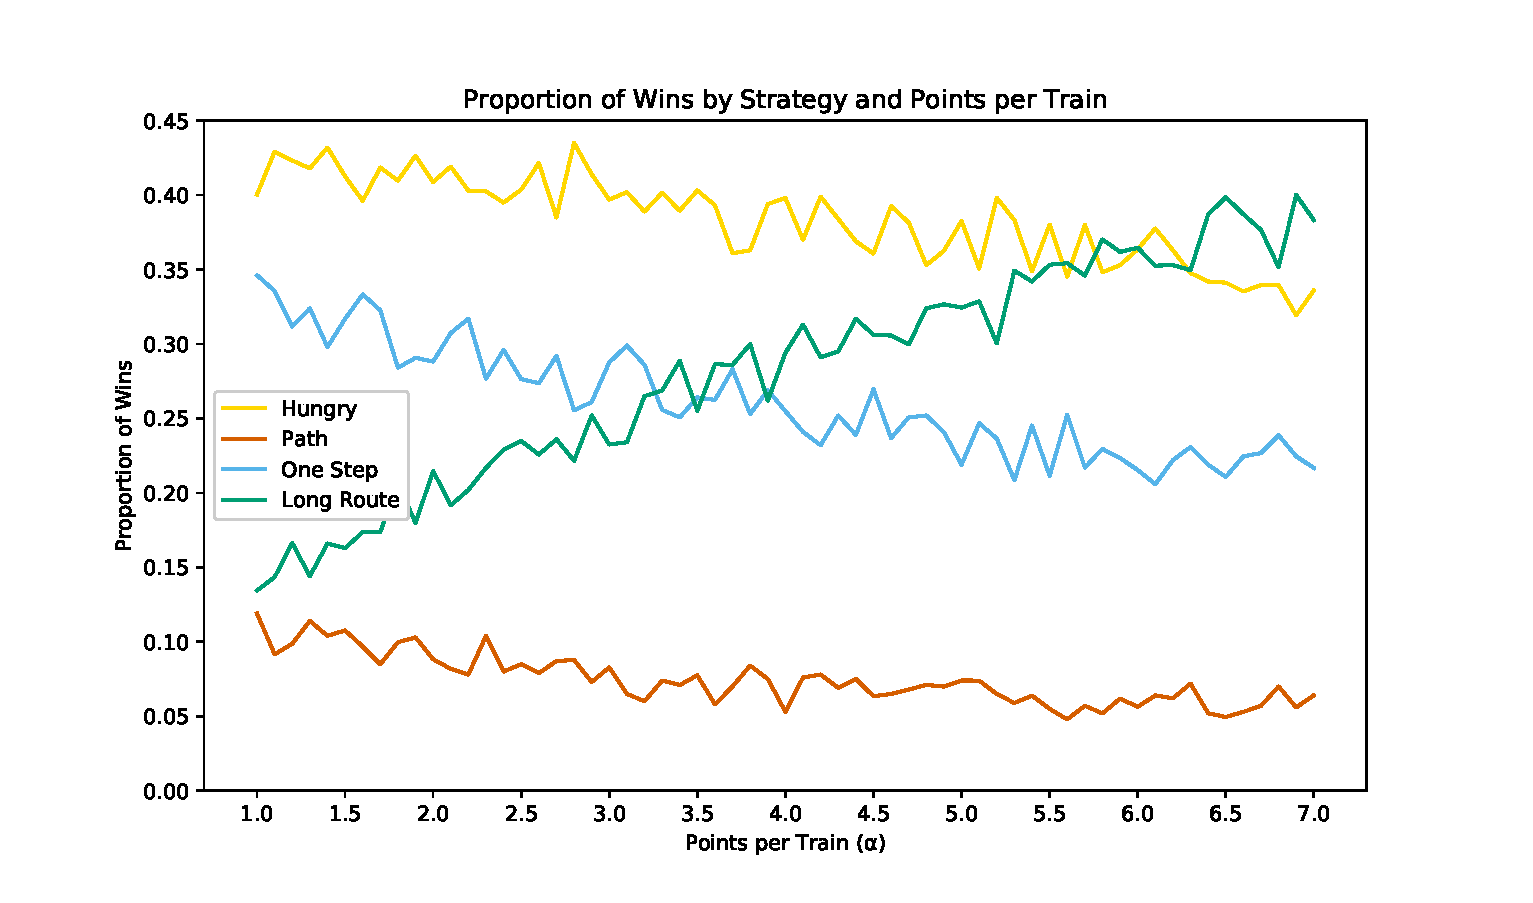
\includegraphics[scale=.65]{figures/points}
    \caption{The proportion of wins
    of each of the four strategies
    by the number of points
    earned per train in 1000 games.}
    \label{fig:points}
\end{figure}
